\subsection{Plotting Hoeffding}

I added the hoeffding bound to the following plot, which now includes all of the bounds including the empirical frequency.

To calculate the hoeffding bound I used $e^{-2 * n * (\epsilon^2)}$, from which I ended up on the following plot of the bound (including the other plots from assignment 1):

\begin{figure}[hbt!]
	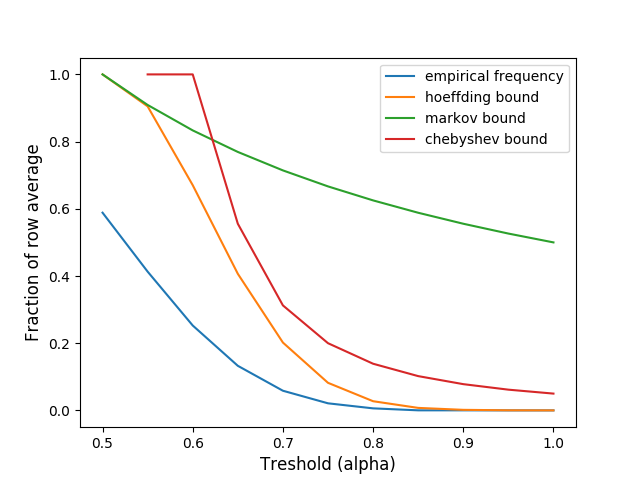
\includegraphics[width=\textwidth]{code/ex1}
	\caption{Plot with all bounds + the empirical frequency}
\end{figure}

\subsection{Compare}
Hoeffding bound overlaps at the beginning with markov but then fastly decreases, even faster then chebyshev which we compared in the first assignment already.
We also can discover that hoeffding gets better with a higher threshold, even better then chebyshev.

\subsection{Exact probability}
From Assignment 1 we have the following probabilities:
So before we got the probability for $\alpha = 0.95$: $\Pr\left[\frac 1 {20} \sum_{i=1}^{20} X_i \geq 0.95 \right] = \frac{21}{1024} \approx 0.0205078125$\\
and for $\alpha = 1$: $\Pr\left[\frac 1 {20} \sum_{i=1}^{20} X_i \geq 1 \right] = \frac 1 {1024} \approx 0.0009765625$

With hoeffding we just need to calculate it by using $e^{-2 * n * (\epsilon^2)}$, for that I directly used my programmed function in python:\\
then we get for $\alpha = 0.95$: $hoeffding(0.5,0.95,20) \approx 0.0003035391380788673$\\
and for $\alpha = 1$: $hoeffding(0.5,1,20) \approx 4.5399929762484854e-05$.\\
So the probabilities lay quite near to each other. Which also gets clear from the plot above, so that hoeffding lands is very near to the exact probability.
Which means for us the hoeffding estimation is very near the exact probability, so outputs quite good results in estimating the probabilities here.